\subsection{Feature Engineering}

Despite the variables provided by original data, we construct some new variables to improve model performance. As we are trying to forecast whether it would precipitate in the next day, the temperature difference in each day could be important. Rain is formatted by condensation of water in air, higher temperature could contribute to evaporation of water and lower temperature may lead to condensation. Therefore, the temperature differences could be useful in predicting precipitation. 

With TMAX (Max temperature in the day) and TMIN in the original data, we construct TDIF = TMAX - TMIN to measure the temperature difference each day. By looking into TDIF in different days we find some interesting phenomena. The overall TDIF is significantly larger in summer than in winter, which can be seen from the range of TDIF in Figure \ref{tdif}. It is also interesting that TDIF at mountain areas is higher than downtown areas in summer, and right the opposite in winter. Those two phenomena indicate the existence of a seasonal pattern in TDIF, and this could be the same for PRCP.

\begin{figure}[h]
\centering
\begin{minipage}[t]{0.48\textwidth}
\centering
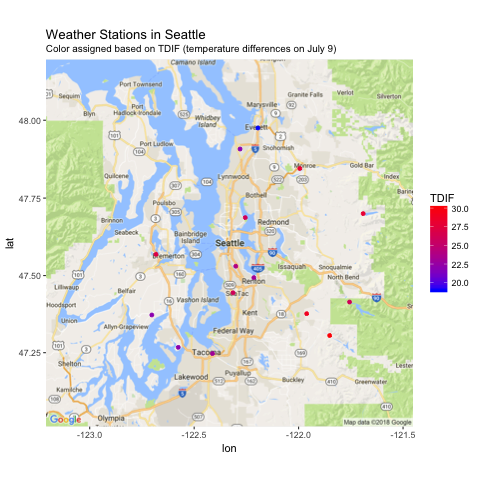
\includegraphics[width=6cm]{tdif1.png}
\end{minipage}
\begin{minipage}[t]{0.48\textwidth}
\centering
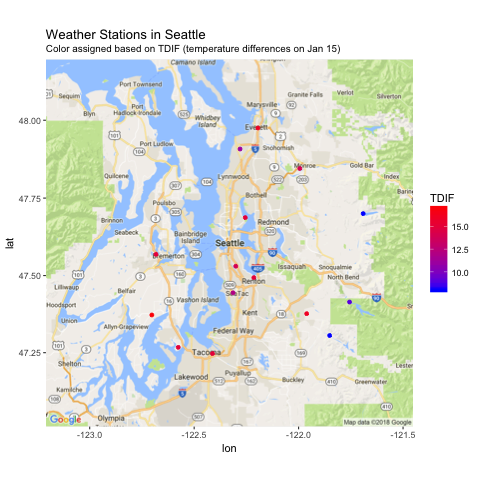
\includegraphics[width=6cm]{tdif2.png}
\end{minipage}
\caption{Stations with TDIF Records}
\label{tdif}
\end{figure}